% !TEX root = main.tex

\section{Google Tango}

Google Tango ist ein Projekt, welches markerlose Augmented-Reality-Applikationen über mehrere Kameras und Tiefensensoren ermöglicht. Bisher sind drei Geräte veröffentlicht worden, welche diese Technologie besitzen. Das erste und zweite Development Kit und das zum Zeitpunkt dieser Seminararbeit bald erscheinende Smartphone von Lenovo. Im folgenden wird hauptsächlich das zweite Development Kit behandelt. Dies ist ein Tablet mit einem 7 Zoll großen Full-HD-Touchscreen-Display, einer 4 MP RGB-IR Kamera kombiniert mit einer 170\degree\/ Kamera mit Bewegungserkennung \cite{tango_teardown}.\par
Der Aufbau und die Wahl der Kameras erinnert stark an die Kinect V2 der Xbox One von Microsoft, sodass die Funktionalität hier sehr ähnlich sein sollte. Der eingebaute Infrarot-Projektor leuchtet den Raum mit einer Vielzahl unsichtbarer Punkte aus. Diese sind unregelmäßig angeordnet, sodass einzigartige Muster entstehen.\par
Die einzige Einschränkung für dieses Verfahren stellen fremde Infrarot-Quellen dar. So ist dies aufgrund der natürlichen Infrarotstrahlung der Sonne nicht bei Tageslicht möglich und mehrere Geräte würden sich untereinander ebenfalls stören. Völlige Dunkelheit stellt jedoch hierfür kein Problem dar.

\subsection{Tiefenmessung und Tracking}
Bevor eine Tiefenmessung oder ein Tracking von Objekten stattfinden kann, muss das Gerät seine eigene Position so genau wie möglich kennen. Dazu wird zum einen die Motion-Tracking-Kamera verwendet. Durch effiziente Analyse z.B. Kanten und Ecken, nimmt diese Bewegung war und kann damit auch feststellen ob sich das Gerät bewegt. Das allein ist jedoch nicht sehr präzise, da sich auch andere Objekte bewegen können. Durch zusätzliche Informationen vom Gyroskop und dem Beschleunigungssensor, welche in vielen Smartphones verbaut sind, kann die genaue Position des Geräts im Raum ermittelt werden \cite{tango_technology}.\par
Um nun die Tiefe von Objekten zu ermitteln kommen drei Systeme zum Einsatz \cite{kinect_imaging}\cite{depth_perception}:
\subsubsection{Structured Light}
Hierbei wird über die Infrarot-Kamera ein Punktmuster ausgesendet. Der Infrarotsensor nimmt dieses und vergleicht es mit seinem virtuellem Abbild. Je größer ein Punkt erscheint, desto weiter ist er entfernt. Dieses Punktmuster ist in Abbildung \ref{tango_ir_projection} zu sehen.
\subsubsection{Time-of-flight}
Es wird ein Infrarot-Strahl ausgesendet. Dieser wird von einem Objekt reflektiert und vom Infrarotsensor aufgenommen. Die Zeit zwischen dem Senden und Empfangen wird dabei gemessen. Je mehr Zeit der Strahl benötigt desto weiter ist der Punkt von dem der Strahl reflektiert wurde entfernt.
\subsubsection{Stereo-Kameras}
Die Szene wird von zwei Kameras aufgenommen. Durch den bekannten Abstand der Kamera und den Kamerawinkeln zum jeweiligen Punkt kann die Tiefe berechnet werden und so eine Tiefenkarte zur aufgenommen Szene erstellt werden.

\begin{figure}[h]
	\centering
	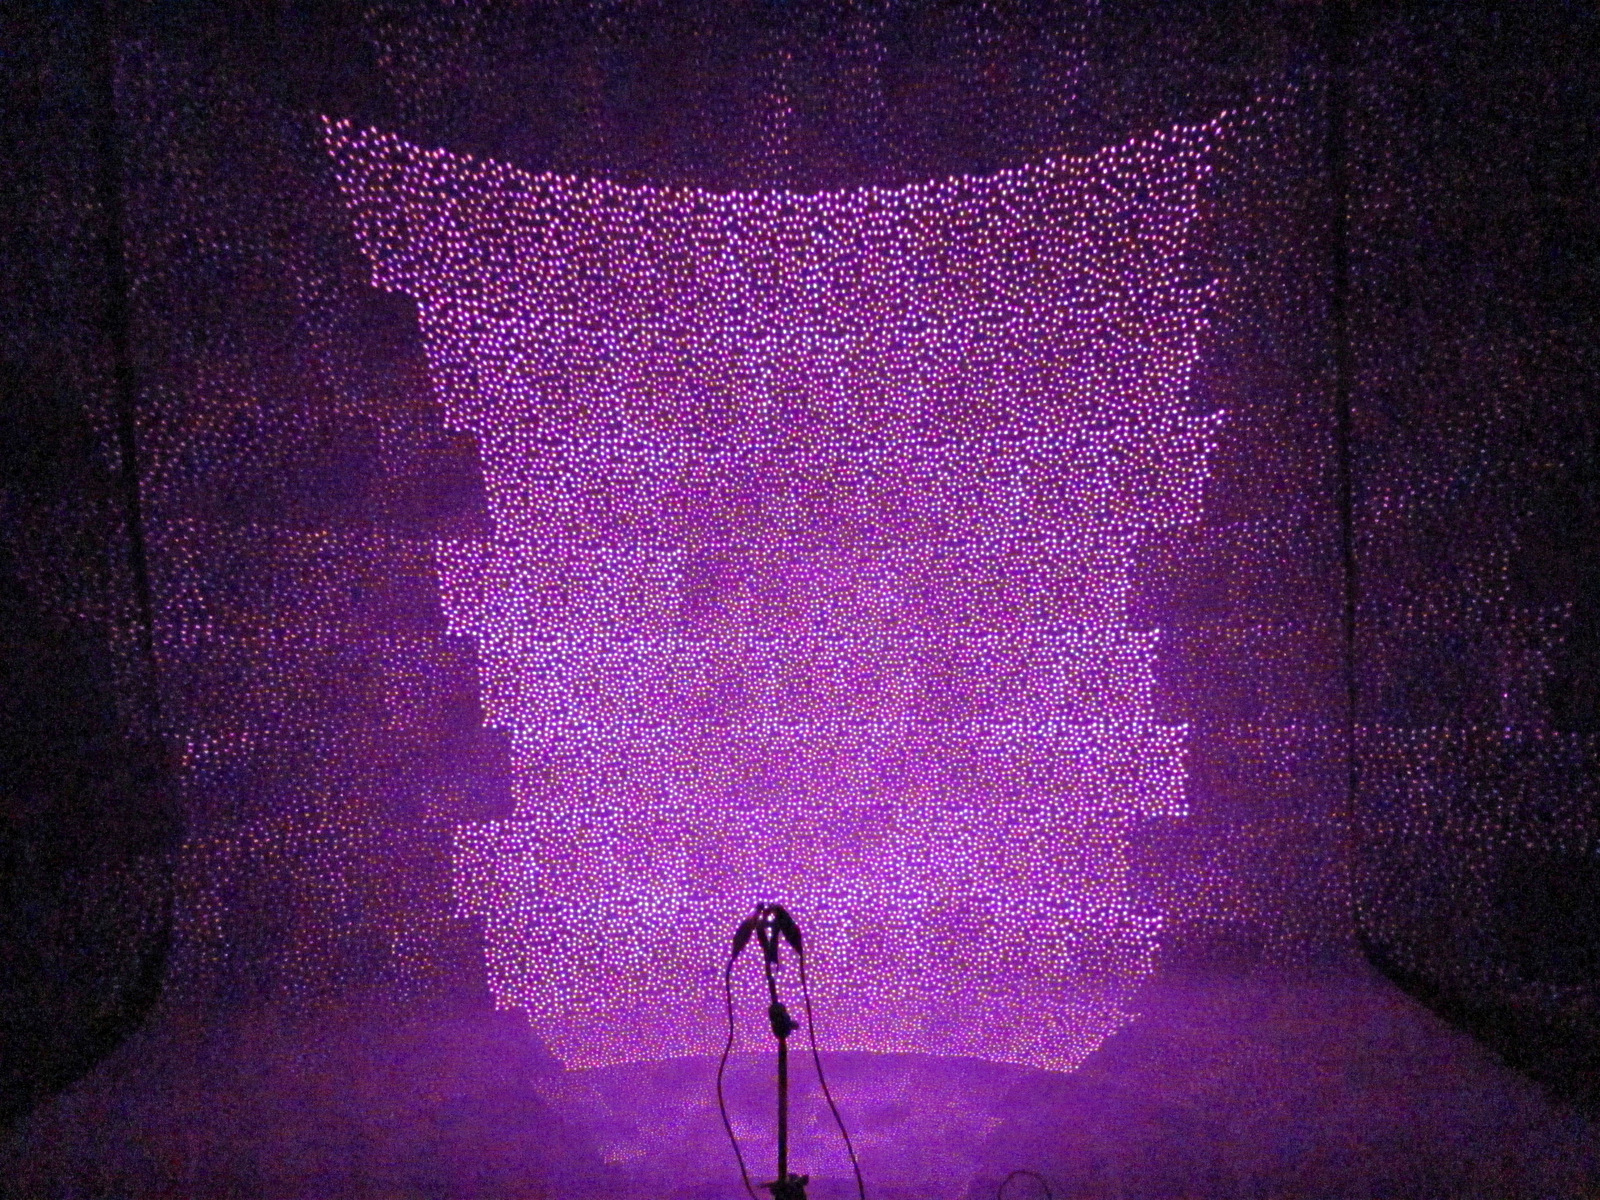
\includegraphics[width=3in]{pictures/tango_ir_projection}
	\caption{Die Umgebung wird mit einem unregelmäßigen Punktmuster per IR-Projektion bestrahlt. (Quelle: \cite{tango_teardown})}
	\label{tango_ir_projection}
\end{figure}

Google Tango liefert die Rohdaten der Technologie als eine sog. "`TangoPointCloud"', welche dann von der eigenen Anwendung verwendet werden kann. Dahinter verbirgt sich im Wesentlichen nichts anderes als ein Array mit allen erfassten Punkten in Form von Koordinaten. Leider ist es mir im Rahmen dieser Arbeit nicht möglich diese Daten selber zu erstellen, da mir die notwendige Hardware zu diesem Zeitpunkt noch nicht zur Verfügung steht.

\subsection{Area Learning \cite{tango_area_learning}}
Diese Rohdaten werden jedoch nicht nur ausgegeben. Sie können durch das Tango Development Kit auch schon verarbeitet werden, um ein "`Gedächtnis"' aufzubauen. Dies nennt sich "`Area Learning"'. Dadurch kann erkannt werden, wann sich das Gerät in einem bekannten Gebiet befindet.\par
Schlüsselelemente der Szene wie Kanten und Ecken werden in einem lokalen Index, dem Area Description File (ADF) gespeichert, um auf diese später wieder zugreifen zu können. Zukünftige Szenen werden dann mit diesen Daten abgeglichen und so kann ungefähr bestimmt werden, wo sich das Gerät bzw. der Nutzer mit dem Gerät befindet. Durch zusätzliche Lokalisierungstechnologien z.B. über WLAN kann das Ergebnis deutlich verbessert werden. Andernfalls können identische Räume, Veränderungen im Raum oder verschiedene Tageszeiten Probleme verursachen. Für letzteres bietet es sich auch an mehrere ADFs zu verwenden, also z.B. eine für die Nacht und eine für den Tag.\par
Des Weiteren soll das Area Learning Fehler des Motion Trackings ausgleichen. Die Position und Ausrichtung des Geräts weicht mit steigender Nutzung von der Position und Ausrichtung, die das Gerät annimmt zu haben, ab. Wenn ein bekanntes Gebiet gefunden wurde, kann dieser Fehler korrigiert werden.

\subsection{Beispielanwendungen \cite{tango_apps}}

\subsubsection{Project Tango Constructor}
Durch diese Anwendung kann die Umgebung mit dem Google Tango-Gerät aufgenommen werden, um daraus ein 3D-Modell zu generieren. Hierbei sind gute Lichtverhältnisse notwendig, sodass die Oberflächen gut abgebildet werden können.

\subsubsection{Project Tango MeasureIt}
Mit dieser Applikation können Strecken auf 2-5\% Genauigkeit \cite{tango_apps} gemessen werden. Für präzise Messungen ist dies ungeeignet, jedoch für die Planung einer Einrichtung o.ä. sollte diese Genauigkeit ausreichend sein. So kann man z.B. einen Türrahmen ausmessen. Solche eine Anwendung der App ist in Abbildung \ref{measure_it} zu sehen
\begin{figure}[h]
	\centering
	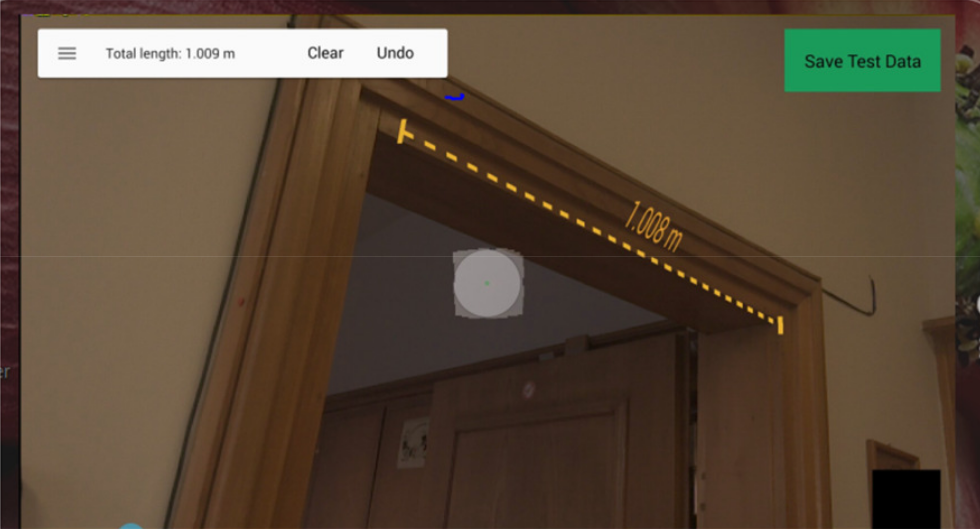
\includegraphics[width=3.25in]{pictures/tango_measure_it}
	\caption{Google Tango App MeasureIt\newline (Quelle: \cite{tango_apps})}
	\label{measure_it}
\end{figure}